\documentclass[a4paper, 14pt]{extarticle}

% Поля
%--------------------------------------
\usepackage{geometry}
\geometry{a4paper,tmargin=2cm,bmargin=2cm,lmargin=3cm,rmargin=1cm}
%--------------------------------------


%Russian-specific packages
%--------------------------------------
\usepackage[T2A]{fontenc}
\usepackage[utf8]{inputenc} 
\usepackage[english, main=russian]{babel}
%--------------------------------------

\usepackage{textcomp}

% Красная строка
%--------------------------------------
\usepackage{indentfirst}               
%--------------------------------------             


%Graphics
%--------------------------------------
\usepackage{graphicx}
\graphicspath{ {./images/} }
\usepackage{wrapfig}
%--------------------------------------

% Полуторный интервал
%--------------------------------------
\linespread{1.3}                    
%--------------------------------------

%Выравнивание и переносы
%--------------------------------------
% Избавляемся от переполнений
\sloppy
% Запрещаем разрыв страницы после первой строки абзаца
\clubpenalty=10000
% Запрещаем разрыв страницы после последней строки абзаца
\widowpenalty=10000
%--------------------------------------

%Списки
\usepackage{enumitem}

%Подписи
\usepackage{caption} 

%Гиперссылки
\usepackage{hyperref}

\hypersetup {
	unicode=true
}

%Рисунки
%--------------------------------------
\DeclareCaptionLabelSeparator*{emdash}{~--- }
\captionsetup[figure]{labelsep=emdash,font=onehalfspacing,position=bottom}
%--------------------------------------

\usepackage{tempora}

%Листинги
%--------------------------------------
\usepackage{listings}
\lstset{
  basicstyle=\ttfamily\footnotesize, 
  %basicstyle=\footnotesize\AnkaCoder,        % the size of the fonts that are used for the code
  breakatwhitespace=false,         % sets if automatic breaks shoulbd only happen at whitespace
  breaklines=true,                 % sets automatic line breaking
  captionpos=t,                    % sets the caption-position to bottom
  inputencoding=utf8,
  frame=single,                    % adds a frame around the code
  keepspaces=true,                 % keeps spaces in text, useful for keeping indentation of code (possibly needs columns=flexible)
  keywordstyle=\bf,       % keyword style
  numbers=left,                    % where to put the line-numbers; possible values are (none, left, right)
  numbersep=5pt,                   % how far the line-numbers are from the code
  xleftmargin=25pt,
  xrightmargin=25pt,
  showspaces=false,                % show spaces everywhere adding particular underscores; it overrides 'showstringspaces'
  showstringspaces=false,          % underline spaces within strings only
  showtabs=false,                  % show tabs within strings adding particular underscores
  stepnumber=1,                    % the step between two line-numbers. If it's 1, each line will be numbered
  tabsize=2,                       % sets default tabsize to 8 spaces
  title=\lstname                   % show the filename of files included with \lstinputlisting; also try caption instead of title
}
%--------------------------------------

%%% Математические пакеты %%%
%--------------------------------------
\usepackage{amsthm,amsfonts,amsmath,amssymb,amscd}  % Математические дополнения от AMS
\usepackage{mathtools}                              % Добавляет окружение multlined
\usepackage[perpage]{footmisc}
%--------------------------------------

%--------------------------------------
%			НАЧАЛО ДОКУМЕНТА
%--------------------------------------

\begin{document}

%--------------------------------------
%			ТИТУЛЬНЫЙ ЛИСТ
%--------------------------------------
\begin{titlepage}
\thispagestyle{empty}
\newpage


%Шапка титульного листа
%--------------------------------------
\vspace*{-60pt}
\hspace{-65pt}
\begin{minipage}{0.3\textwidth}
\hspace*{-20pt}\centering

\includegraphics[width=\textwidth]{emblem}
\end{minipage}
\begin{minipage}{0.67\textwidth}\small \textbf{
\vspace*{-0.7ex}
\hspace*{-6pt}\centerline{Министерство науки и высшего образования Российской Федерации}
\vspace*{-0.7ex}
\centerline{Федеральное государственное бюджетное образовательное учреждение }
\vspace*{-0.7ex}
\centerline{высшего образования}
\vspace*{-0.7ex}
\centerline{<<Московский государственный технический университет}
\vspace*{-0.7ex}
\centerline{имени Н.Э. Баумана}
\vspace*{-0.7ex}
\centerline{(национальный исследовательский университет)>>}
\vspace*{-0.7ex}
\centerline{(МГТУ им. Н.Э. Баумана)}}
\end{minipage}
%--------------------------------------

%Полосы
%--------------------------------------
\vspace{-25pt}
\hspace{-35pt}\rule{\textwidth}{2.3pt}

\vspace*{-20.3pt}
\hspace{-35pt}\rule{\textwidth}{0.4pt}
%--------------------------------------

\vspace{1.5ex}
\hspace{-35pt} \noindent \small ФАКУЛЬТЕТ\hspace{80pt} <<Информатика и системы управления>>

\vspace*{-16pt}
\hspace{47pt}\rule{0.83\textwidth}{0.4pt}

\vspace{0.5ex}
\hspace{-35pt} \noindent \small КАФЕДРА\hspace{50pt} <<Теоретическая информатика и компьютерные технологии>>

\vspace*{-16pt}
\hspace{30pt}\rule{0.866\textwidth}{0.4pt}
  
\vspace{11em}

\begin{center}
\Large {\bf Лабораторная работа № 1} \\ 
\large {\bf по курсу <<Компьютерные сети>>} \\
\large <<Простейший протокол прикладного уровня>> 
\end{center}\normalsize

\vspace{8em}


\begin{flushright}
  {Студент группы ИУ9-32Б Волохов А. В. \hspace*{15pt}\\ 
  \vspace{2ex}
  Преподаватель Посевин Д. П.\hspace*{15pt}}
\end{flushright}

\bigskip

\vfill
 

\begin{center}
\textsl{Москва 2023}
\end{center}
\end{titlepage}
%--------------------------------------
%		КОНЕЦ ТИТУЛЬНОГО ЛИСТА
%--------------------------------------

\renewcommand{\ttdefault}{pcr}

\setlength{\tabcolsep}{3pt}
\newpage
\setcounter{page}{2}
\section{Задание}\label{Sect::task}
Целью работы является знакомство с принципами разработки протоколов прикладного уровня и их реализацией на языке Go. 
Необходимо реализовать протокол редактирования предложения с возможностью вставлять и удалять слова
Исходный код программы представлен в листингах~\ref{lst:code1}--~\ref{lst:code2}--~\ref{lst:code3}--~\ref{lst:code4}--~\ref{lst:code5}--~\ref{lst:code6}.

\begin{figure}[!htb]
\begin{lstlisting}[language={Go},caption={proto.go},label={lst:code1}]
package proto

import "encoding/json"

type Request struct {
	Command string `json:"command"`
	Data *json.RawMessage `json:"data"`
}

type Response struct {
	Status string `json:"status"`
	Data *json.RawMessage `json:"data"`
}

type Word struct {
	Word string `json:"word"`
	Key string `json:"num"`
}

\end{lstlisting}
\end{figure}

\newpage

\begin{figure}[!htb]
\begin{lstlisting}[language={Go},caption={server.go},label={lst:code2}]
package main

import (
	"encoding/json"
	"flag"
	"fmt"
	"github.com/mgutz/logxi/v1"
	"net"
	"strings"
)

import "file/lab1/src/proto"

type Client struct {
	logger log.Logger       
	conn   *net.TCPConn      
	enc    *json.Encoder     
	sent   map[string]string 
}

func NewClient(conn *net.TCPConn) *Client {
	return &Client{
		logger: log.New(fmt.Sprintf("client %s", conn.RemoteAddr().String())),
		conn:   conn,
		enc:    json.NewEncoder(conn),
		sent:   make(map[string]string),
	}
}

func (client *Client) serve() {
	defer client.conn.Close()
	decoder := json.NewDecoder(client.conn)
	for {
		var req proto.Request
		if err := decoder.Decode(&req); err != nil {
			client.logger.Error("cannot decode message", "reason", err)
			break
		} else {
			client.logger.Info("received command", "command", req.Command)
			if client.handleRequest(&req) {
				client.logger.Info("shutting down connection")
				break
			}
		}
	}
}


\end{lstlisting}
\end{figure}

\newpage
\begin{figure}[!htb]
\begin{lstlisting}[language={Go},caption={server.go - продолжение},label={lst:code3}]
func (client *Client) handleRequest(req *proto.Request) bool {
	switch req.Command {
	case "quit":
		client.respond("ok", nil)
		return true
	case "add":
		errorMsg := ""
		if req.Data == nil {
			errorMsg = "data field is absent"
		} else {
			var word proto.Word
			if err := json.Unmarshal(*req.Data, &word); err != nil {
				errorMsg = "malformed data field"
			} else {
				client.logger.Info("adding a word", "value", word.Word, "key", word.Key)
				client.sent[word.Key] = word.Word
			}
		}
		if errorMsg == "" {
			client.respond("ok", nil)
		} else {
			client.logger.Error("adding failed", "reason", errorMsg)
			client.respond("failed", errorMsg)
		}
	case "del":
		if req.Data == nil {
			client.logger.Error("deletion failed", "reason", "key is missing in data field")
			client.respond("failed", "key is missing in data field")
		} else {
			keyToDelete := strings.Trim(string(*req.Data), "\"")
			deletedWord, ok := client.sent[keyToDelete]
			if ok {
				delete(client.sent, keyToDelete)
				client.respond("result", &proto.Word{
					Key:  keyToDelete,
					Word: deletedWord,
				})
			} else {
				client.logger.Error("deletion failed", "reason", "key not found")
				client.respond("failed", "key not found")
			}
		}
	case "sent":
		concatenatedValues := ""
		for _, value := range client.sent {
			concatenatedValues += value + " "
		}
		client.respond("result", &proto.Word{
			Key:  "sentence",
			Word: concatenatedValues,
		})

	
\end{lstlisting}
\end{figure}
\newpage
\begin{figure}[!htb]
\begin{lstlisting}[language={Go},caption={server.go - продолжение},label={lst:code4}]
default:
		client.logger.Error("unknown command")
		client.respond("failed", "unknown command")
	}
	return false
}

func (client *Client) respond(status string, data interface{}) {
	var raw json.RawMessage
	raw, _ = json.Marshal(data)
	client.enc.Encode(&proto.Response{status, &raw})
}

func main() {
	var addrStr string
	flag.StringVar(&addrStr, "addr", "127.0.0.1:6000", "specify ip address and port")
	flag.Parse()

	if addr, err := net.ResolveTCPAddr("tcp", addrStr); err != nil {
		log.Error("address resolution failed", "address", addrStr)
	} else {
		log.Info("resolved TCP address", "address", addr.String())

		if listener, err := net.ListenTCP("tcp", addr); err != nil {
			log.Error("listening failed", "reason", err)
		} else {
			for {
				if conn, err := listener.AcceptTCP(); err != nil {
					log.Error("cannot accept connection", "reason", err)
				} else {
					log.Info("accepted connection", "address", conn.RemoteAddr().String())

					go NewClient(conn).serve()
				}
			}
		}
	}
}
\end{lstlisting}
\end{figure}
\newpage
\begin{figure}[!htb]
\begin{lstlisting}[language={Go},caption={client.go},label={lst:code5}]
package main

import (
	"encoding/json"
	"flag"
	"fmt"
	"github.com/skorobogatov/input"
	"net"
)

import "file/lab1/src/proto"

func interact(conn *net.TCPConn) {
	defer conn.Close()
	encoder, decoder := json.NewEncoder(conn), json.NewDecoder(conn)
	for {
		fmt.Printf("command = ")
		command := input.Gets()
		switch command {
		case "quit":
			send_request(encoder, "quit", nil)
			return
		case "add":
			var word proto.Word
			fmt.Printf("word = ")
			word.Word = input.Gets()
			fmt.Printf("key = ")
			word.Key = input.Gets()
			send_request(encoder, "add", &word)
		case "del":
			fmt.Printf("key = ")
			var key = input.Gets()
			send_request(encoder, "del", key)
		case "sent":
			send_request(encoder, "sent", nil)
		default:
			fmt.Printf("error: unknown command\n")
			continue
		}
		var resp proto.Response
		if err := decoder.Decode(&resp); err != nil {
			fmt.Printf("error: %v\n", err)
			break
		}
\end{lstlisting}
\end{figure}

\newpage

\begin{figure}[!htb]
\begin{lstlisting}[language={Go},caption={client.go - продолжение},label={lst:code6}]
switch resp.Status {
		case "ok":
			fmt.Printf("ok\n")
		case "failed":
			if resp.Data == nil {
				fmt.Printf("error: data field is absent in response\n")
			} else {
				var errorMsg string
				if err := json.Unmarshal(*resp.Data, &errorMsg); err != nil {
					fmt.Printf("error: malformed data field in response\n")
				} else {
					fmt.Printf("failed: %s\n", errorMsg)
				}
			}
		case "result":
			if resp.Data == nil {
				fmt.Printf("error: data field is absent in response\n")
			} else {
				var word proto.Word
				if err := json.Unmarshal(*resp.Data, &word); err != nil {
					fmt.Printf("error: malformed data field in response\n")
				} else {
					fmt.Printf("result: word \"%s\" with key = %s \n", word.Word, word.Key)
				}
			}
		default:
			fmt.Printf("error: server reports unknown status %q\n", resp.Status)
		}
	}
}
func send_request(encoder *json.Encoder, command string, data interface{}) {
	var raw json.RawMessage
	raw, _ = json.Marshal(data)
	encoder.Encode(&proto.Request{command, &raw})
}

func main() {
	var addrStr string
	flag.StringVar(&addrStr, "addr", "127.0.0.1:6000", "specify ip address and port")
	flag.Parse()
	if addr, err := net.ResolveTCPAddr("tcp", addrStr); err != nil {
		fmt.Printf("error: %v\n", err)
	} else if conn, err := net.DialTCP("tcp", nil, addr); err != nil {
		fmt.Printf("error: %v\n", err)
	} else {
		interact(conn)
	}
}

\end{lstlisting}
\end{figure}

\newpage

\begin{figure}[!htb]
	\centering
	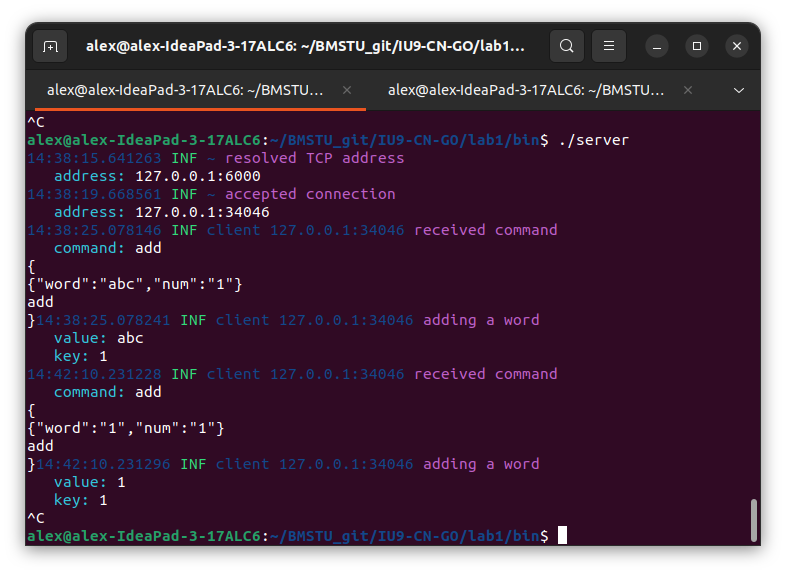
\includegraphics[width=0.8\textwidth]{res1.png}
\caption{Сервер}
\label{fig:img1}
\end{figure}
\begin{figure}[!htb]
	\centering
	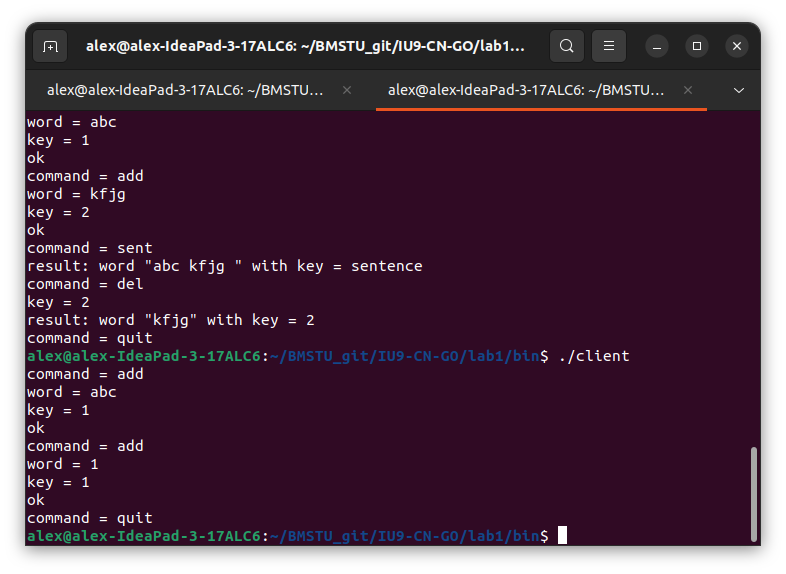
\includegraphics[width=0.8\textwidth]{res2.png}
\caption{Клиент}
\label{fig:img2}
\end{figure}





\end{document}
